% Sinh boi runners/make_paper1_figures.py; caption doi chieu bang
% runners/audit_figures.py. File rieng cho tung hinh de \input DUNG CHO
% trong than bai -- float cua LaTeX chi troi VE SAU, khai bao het o cuoi
% tai lieu thi ca 9 hinh don xuong cuoi va tran vao danh muc tai lieu.

\begin{figure*}[t]
  \centering
  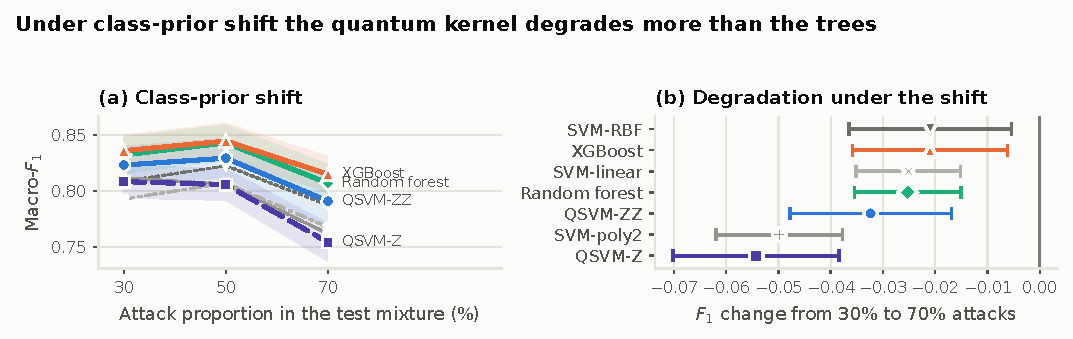
\includegraphics[width=\textwidth]{figs_revision/fig8_prior_shift.pdf}
  \caption{%
    \textbf{Under class-prior shift the quantum kernel degrades more than the
    tree ensembles, not less.} (a) Macro-$F_1$ as the attack proportion moves
    from $30\%$ to $70\%$, over ten runs with $95\%$ bands. (b) The paired
    change across that shift, sorted. \QSVM{} loses $0.032$ against $0.021$ for
    XGBoost and $0.025$ for the random forest. The submitted version named this
    regime as its strongest evidence.}
  \label{fig:priorshift}
\end{figure*}
